
%%%%%%%%%%%%%%%%%%%%%%%%%%%%%%%%%%
%\noindent {\bf Introduction}\\
In this note we assess the sensitivity of vector boson scattering (VBS) processes to different dimension-6 ($\mathrm{dim=6}$) operators. We focus here on the $ZZ$ final state, decaying to 4 charged leptons. This experimental channel, currently statistically limited at the LHC \cite{Sirunyan:2017fvv}, will become more interesting at the HL-LHC because of the attainable selection purity. The full reconstruction of the final states also gives access to cleaner observables with respect to final states involving $W$ bosons, where neutrino 4-momenta must be inferred using approximated methods.
This analysis can nevertheless be repeated analogously to other VBS final states. 

In \cite{Gomez-Ambrosio:2018pnl} we studied the purely electroweak component of the $p p \to Z Z j j$ process, referred to as VBS(ZZ). Sensitivity to several $\mathrm{dim=6}$ operators has been demonstrated, as well as the impact of such EFT contribution on the VBS cross-section and triple and quartic gauge couplings (TGCs and QGCs). 

Here we update predictions for the HL-LHC setup and show the kinematic distributions for a handful of relevant operators. For the $\mathrm{dim=6}$ parametrisations we use the \emph{Warsaw basis} from \cite{Grzadkowski:2010es}, following the notation and classification from \cite{Jenkins:2013zja}. Other technical details can be found in the original publication \cite{Gomez-Ambrosio:2018pnl}.

\begin{figure}[h!]
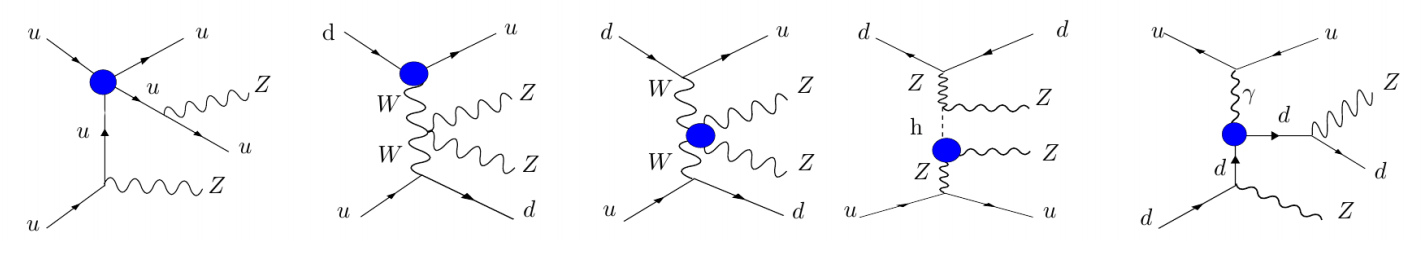
\includegraphics[scale=0.3]{\main/section4/plots/feynmandiagramssignal.png}
\caption{Examples of some EFT diagrams for the VBS(ZZ) signal. The blobs represent $\mathrm{dim=6}$ insertions.}
\end{figure}

%{\large{\bf Effective Field Theory parametrization}} \\ \\
\noindent {\bf Effective Field Theory parametrisation}\\
%
We consider the standard SMEFT parametrisation of eq.~(\ref{EFTLAG}).\footnote{In particular, we assume CP symmetry, neglecting the CP-odd operators since their impact on VBS cross-sections and differential distributions is negligible. However it is well known that certain variables of these processes (namely spin correlations and polarisations) can be sensible to CP-violation.} Further, the SMEFT amplitudes and cross sections can be parametrised as
%
\begin{equation}
\mathcal{A}_{EFT} = \mathcal{A}_{SM} + \frac{g'}{\Lambda^2} \mathcal{A}_{6} +   \frac{g'^2}{\Lambda^4} \mathcal{A}_{8} + \dots 
\end{equation}
%
\begin{equation}
 \sigma_{EFT} \sim \vert \mathcal{A}_{SM} \vert^2 + {\color{red} 2\frac{g'}{\Lambda^2} \mathcal{A}_{SM} \mathcal{A}_{6} } + {\color{blue} \frac{g'2}{\Lambda^4} \left(  2 \mathcal{A}_{SM} \mathcal{A}_{8} + \vert \mathcal{A}_{6} \vert^2 \right)} + \dots
\end{equation}
%
Here, we assume the linear contribution (red) of the EFT effects to be leading. Analysis of the $\mathrm{dim=6}$ quadratic terms and the $\mathrm{dim=8}$ interference terms (both in blue) will be subject of further studies.  In particular, $\mathrm{dim=8}$ are commonly associated with quartic gauge couplings and such contribution, albeit sub-leading, would represent some added value to the linear $\mathrm{dim=6}$ prediction. \\
 
\noindent {\bf Definition of the fiducial region}\\
The VBS(ZZ) process has a very peculiar experimental signature, with two energetic forward jets and 4 identifiable charged leptons ($\ell, \ell' = \mu$ or $e$).
The electroweak component of the process $p p \to Z Z j j \to \ell \bar{\ell} \, \ell' \bar{\ell'} j j$ is defined and isolated through some experimental cuts. The ones used in the CMS analysis (in the measurement of the fiducial cross-section) can be found in \cite{Sirunyan:2017fvv}. Here we define a similarly VBS-enriched region, with a relaxed $m_{jj}$ selection: %{\color{red} Editors, I'd like to have this in 2 columns but I don't want to mess up anything.... usepackage{multicol} didnt work unfortunately}
%
%\begin{multicols}{2}
\begin{eqnarray}
p_T (j) > 30 \textrm{\UGeV} \quad \Delta \eta (j_1 j_2) > 2.4\quad m_{jj} > 100 \textrm{\UGeV}\quad \textrm{\emph{on-shell}}Z_1,Z_2
\end{eqnarray}
%\end{multicols}
%

%%%%%%%%%%%%%%%%%%%%%%%%%%%%%%%%%%%%%%%%%%%%%%%%%%%%%5
 
 
\noindent {\bf EFT analysis}\\ 
In tables~\ref{tab:signal} and \ref{tab:background} we show the sensitivities to different $\mathrm{dim=6}$ operators of the VBS(ZZ) process, as well as of its main background at LHC: the di-boson production channel from quark-antiquark annihilation associated to gluon radiation (studied in depth by CMS for LHC runs I and II in \cite{Sirunyan:2018vkx}, QCD(ZZ)). 

Further, in figure \ref{fig:plots} we show differential distributions for a subset of operators. In particular we chose the three operators that directly affect triple and quartic gauge couplings, with the following notation, which differs from that of table~\ref{tab:dim6ops},
%\begin{multicols}{2}
\begin{equation}
\mathcal{O}_W = \frac{3!}{g}\mathcal{O}_{3W}\quad
\mathcal{O}_{HW} = \frac{1}{g^2}\mathcal{O}_{WW}\quad
\mathcal{O}_{HWB} = \frac{1}{gg^\prime}\mathcal{O}_{WB}
\end{equation}
However, as reported in tables~\ref{tab:signal} and \ref{tab:background}, there are other relevant operators for the VBS process, 
% in general and the TGC and QGC in particular. 
for example $\mathcal{O}_{\ell \ell}$, the 4-lepton operator that affects $G_F$, or $\mathcal{O}_{HB}$ that enters the $Z$ boson propagator. More details can be found for example in \cite{Ghezzi:2015vva}.
 
Figure \ref{fig:plots} should be interpreted as follows: we select one paradigmatic operator (for example $\mathcal{O}_W$), and see how much does its interference term affect the VBS and di-boson signals ($2.5\%$ in this case). As the VBS(ZZ) cross section is still mostly unconstrained experimentally, while the QCD(ZZ) has a $21\%$ uncertainty in the 2-jet bin \cite{Sirunyan:2018vkx}, we know the bounds within which we can vary this coefficient. If we assume for example a $10 \%$ positive interference with the total cross-section, we observe that such a small contribution to the total cross-section can represent a large modification in certain bins of the differential distributions. This advantage is twofold: with this procedure we can select the optimal bin(s) for the study and fit of each EFT operator; and, by applying unitarity considerations, we can constrain the values of the Wilson coefficients further. In our example, a contribution of $10 \%$ in $\mathcal{O}_W$, still allowed for the total rate, has a large impact on the high energy bins of the $p_T (Z_1)$ distribution. 
\\
 
\noindent {\bf Conclusions}\\
The VBS(ZZ) and QCD(ZZ) final states, still largely unexplored at the LHC, will be an important source of constraints on $\mathrm{dim=6}$ EFT operators at the HL-LHC. We have shown the impact that values of Wilson coefficients still experimentally allowed have on differential distributions that are easily accessible experimentally in this channel. 

% 
\begin{figure}[htbp]
  \begin{minipage}[b]{0.5\textwidth}
    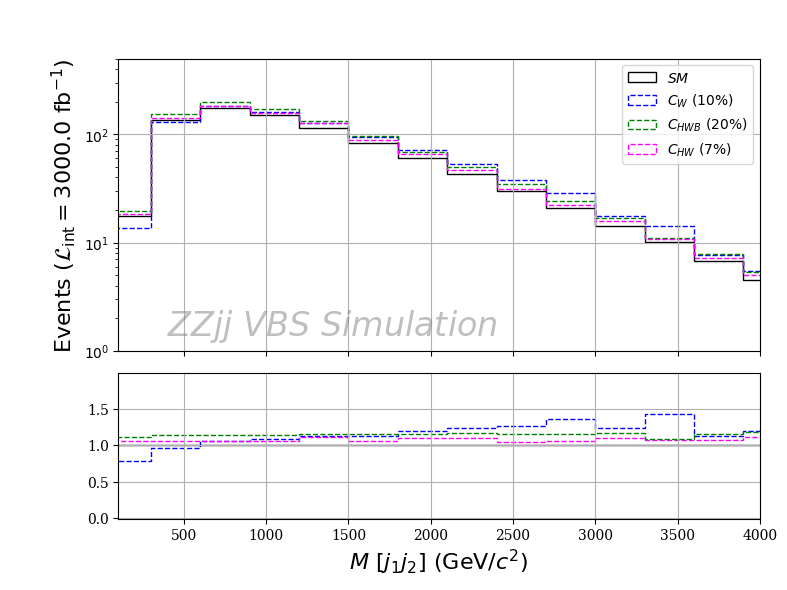
\includegraphics[width=1.02\textwidth]{\main/section4/plots/mjj.png}
    %\caption{Picture 1}
    %\label{fig:1}
  \end{minipage}
  %
  \begin{minipage}[b]{0.5\textwidth}
    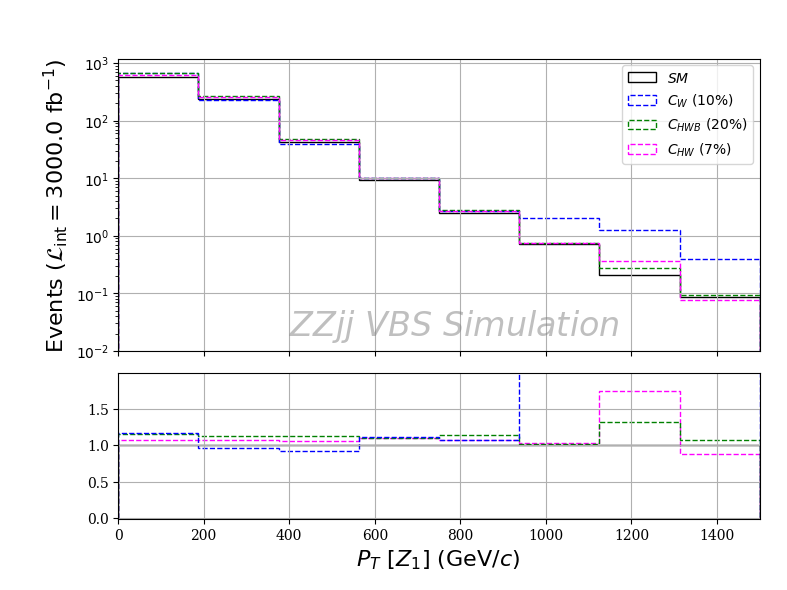
\includegraphics[width=1.02\textwidth]{\main/section4/plots/ptz.png}
    %\caption{Picture 2}
    %\label{fig:2}
  \end{minipage}
  \caption{Two generic simulations showing the EFT effects on key differential distributions: invariant mass of the di-jet system (left) and transverse momentum of the leading Z boson (right). We selected arbitrary values for the Wilson coefficients $\lbrace c_W, c_{HW}, c_{HWB} \rbrace$. Notice that the notation differs from table \ref{tab:dim6ops}.}
  \label{fig:plots}
\end{figure}

%%%%%%%%%%%%%%%%%%%%%%%%%%%%%%%%%%%%%%%%%%%%%%%%%%%%%%%%%%%%%%%%%%

\begin{table*}[]
\begin{center}
\small
\begin{tabular}{|c|c|}%\hline
\hline
VBS Signal & Signal strengths (Linear EFT) \\
\hline
%\hline
 Class 1:  &  $\mathcal{O}_W = c_W \cdot 2.5 \%$ \\
 Class 3: & $\mathcal{O}_{HD} = c_{HD} \cdot 6.0 \%$ \\
 Class 4: & $ \mathcal{O}_{HW} = c_{HW} \cdot 5 \% $, $ \mathcal{O}_{CHB} = c_{HB} \cdot 0.2 \% $,  $ \mathcal{O}_{HWB} = c_{HWB} \cdot 14 \% $\\
 Class 7: & $ \mathcal{O}_{Hl^{(3)}} = c_{Hl^{(3)}} \cdot 48 \% $,
 $ \mathcal{O}_{Hq^{(1)}} = c_{Hq^{(1)}} \cdot 2 \% $, \\ 
 & $ \mathcal{O}_{Hq^{(3)}} = c_{Hq^{(3)}} \cdot 46 \% $,  $ \mathcal{O}_{Hu} = c_{Hu} \cdot 0.8 \% $ 
 \\
 Class 8a: $(L \bar{L})(L \bar{L})$  &  ($G_F \to$) $ \mathcal{O}_{\ell \ell} = c_{\ell \ell} \cdot 24 \% $ , 
 $ \mathcal{O}_{qq^{(1)}} = c_{qq^{(1)}} \cdot 12 \% $, \\ &
$ \mathcal{O}_{qq^{(11)}} = c_{qq^{(11)}} \cdot 14 \% $, 
$ \mathcal{O}_{qq^{(33)}} = c_{qq^{(33)}} \cdot 100 \% $, 
$ \mathcal{O}_{qq^{(31)}} = c_{qq^{(31)}} \cdot 75 \% $
 \\
\hline 
 \end{tabular}
  \caption{  Different sensitivities to each of the Warsaw basis operators. The operators that are not listed do not intervene in the process, or do it in a negligible way. Each sensitivity $\epsilon_i$ is calculated as $\epsilon_i  = \vert \frac{\sigma_{EFT} - \sigma_{SM}}{\sigma_{SM}} \vert$, and they include a standard EFT pre-factor $\frac{v^2}{\Lambda^2}\vert_{\Lambda=1\UTeV}$ which needs to be taken into account if substituting values for the $c_i$ in the table. NB: we quote the absolute value for the sensitivities $\epsilon$. Notice that the notation differs from table \ref{tab:dim6ops}.}
  \label{tab:signal}
\end{center}
\end{table*}


\begin{table*}[]
\begin{center}
\small
\begin{tabular}{|c|c|}%\hline
\hline
ZZ Di-boson & Sensitivities (Linear EFT) \\
\hline
%\hline
 Class 1:  &  $\mathcal{O}_G = 2.5 \%$, \quad $\mathcal{O}_W = 2.5 \%$ \\
Class 3: & $\mathcal{O}_{HD} = 6.0 \%$ \\
Class 4: & $ \mathcal{O}_{CHW} = 0.2 \% $, $ \mathcal{O}_{CHG} =  8 \% $, $ \mathcal{O}_{CHB} =  0 \% $, $ \mathcal{O}_{CHWB} =  12 \% $ \\
Class 7: & $ \mathcal{O}_{Hl^{(3)}} = c_{Hl^{(3)}} \cdot 25 \% $ ,
$ \mathcal{O}_{Hq^{(1)}} = c_{Hq^{(1)}} \cdot 3 \% $, \\ & 
$ \mathcal{O}_{Hq^{(3)}} = c_{Hq^{(3)}} \cdot 31 \% $,
$ \mathcal{O}_{Hu} = c_{Hu} \cdot 1.1 \% $
%,$ \mathcal{O}_{Hu} = c_{Hd} \cdot 0.1 \% $
\\
Class 8a: $(L \bar{L})(L \bar{L})$  &  ($G_F \to$) $ \mathcal{O}_{\ell \ell} = c_{\ell \ell} \cdot 12 \% $ , $ \mathcal{O}_{qq^{(1)}} = c_{qq^{(1)}} \cdot 1.0 \% $, \\ &
$ \mathcal{O}_{qq^{(11)}} = c_{qq^{(11)}} \cdot 1.3 \% $, 
$ \mathcal{O}_{qq^{(33)}} = c_{qq^{(33)}} \cdot 8.4 \% $, 
$ \mathcal{O}_{qq^{(31)}} = c_{qq^{(31)}} \cdot 8.0 \% $
\\
\hline
 \end{tabular}
  \caption{Sensitivities to the different $\mathrm{dim=6}$ operators in the di-boson production channel, main background for the VBS(ZZ) at LHC. A large sensitivity does not necessarily mean that a large EFT effect is expected, since the corresponding Wilson coefficient might as well be very small. Notice that the notation differs from table \ref{tab:dim6ops}. %NB: we quote the absolute value for the sensitivities $\epsilon$.  
  }
  \label{tab:background}
\end{center}
\end{table*}